\documentclass{chi-ext}
% Please be sure that you have the dependencies (i.e., additional LaTeX packages) to compile this example.
% See http://personales.upv.es/luileito/chiext/

%% EXAMPLE BEGIN -- HOW TO OVERRIDE THE DEFAULT COPYRIGHT STRIP -- (July 22, 2013 - Paul Baumann)
% \copyrightinfo{Permission to make digital or hard copies of all or part of this work for personal or classroom use is granted without fee provided that copies are not made or distributed for profit or commercial advantage and that copies bear this notice and the full citation on the first page. Copyrights for components of this work owned by others than ACM must be honored. Abstracting with credit is permitted. To copy otherwise, or republish, to post on servers or to redistribute to lists, requires prior specific permission and/or a fee. Request permissions from permissions@acm.org. \\
% {\emph{CHI'14}}, April 26--May 1, 2014, Toronto, Canada. \\
% Copyright \copyright~2014 ACM ISBN/14/04...\$15.00. \\
% DOI string from ACM form confirmation}
%% EXAMPLE END -- HOW TO OVERRIDE THE DEFAULT COPYRIGHT STRIP -- (July 22, 2013 - Paul Baumann)

\title{FeedLearn: Using Social Feeds for Microlearning}

\numberofauthors{1}
% Notice how author names are alternately typesetted to appear ordered in 2-column format;
% i.e., the first 4 autors on the first column and the other 4 auhors on the second column.
% Actually, it's up to you to strictly adhere to this author notation.
\author{
  \alignauthor{
  	\textbf{Geza Kovacs}\\
  	\affaddr{Department of Computer Science, Stanford University}\\
  	\email{geza@cs.stanford.edu}
  }
}

% Paper metadata (use plain text, for PDF inclusion and later re-using, if desired)
\def\plaintitle{FeedLearn: Using Social Feeds for Microlearning}
\def\plainauthor{Geza Kovacs}
\def\plainkeywords{microlearning, social feeds, language learning}
\def\plaingeneralterms{microlearning, social feeds, language learning}

\hypersetup{
  % Your metadata go here
  pdftitle={\plaintitle},
  pdfauthor={\plainauthor},  
  pdfkeywords={\plainkeywords},
  pdfsubject={\plaingeneralterms},
  % Quick access to color overriding:
  %citecolor=black,
  %linkcolor=black,
  %menucolor=black,
  %urlcolor=black,
}

\usepackage{graphicx}   % for EPS use the graphics package instead
\usepackage{balance}    % useful for balancing the last columns
\usepackage{bibspacing} % save vertical space in references

\usepackage{paralist}

%\usepackage{tikz}
\usepackage[absolute]{textpos}
%\usepackage{float}

\begin{document}

\maketitle

\begin{textblock}{5}(3.6,7.7)
\begin{figure}
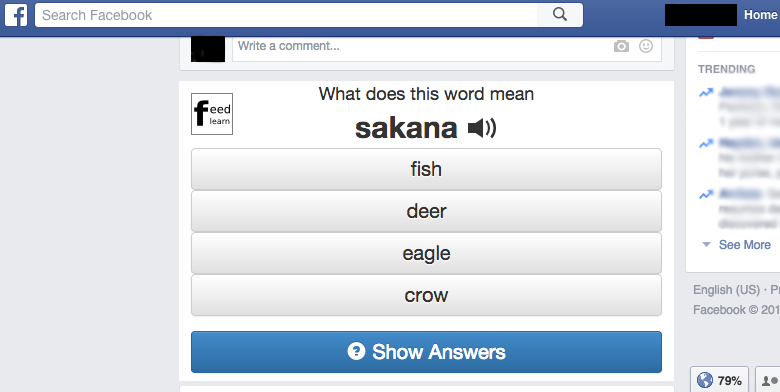
\includegraphics[width=\columnwidth]{feedlearn-screenshot.png}
\caption{FeedLearn showing an interactive vocabulary quiz inside a user's Facebook news feed}
\end{figure}
\end{textblock}

\begin{abstract}
Many long-term goals, such as learning a new language,
require the person to spend a small amount of time each day to achieve them.
At the same time, people regularly browse social news feeds in their spare time.
Our system, FeedLearn, exploits the regularity with which people spend their time reading news feeds on Facebook,
in order to present them with vocabulary quizzes they can answer directly inside the feed.
It is implemented as a Chrome extension, as Facebook's API does not currently allow such flexible
in-feed interactions.
In our preliminary user study, we find that over the course of 2 weeks, we are able to teach students an average of 11 new vocabulary words by injecting microlearning tasks into their Facebook feeds. This is twice as much the 5 vocabulary words learned if we insert reminders to visit an external site and study, as is done by current Facebook apps.
% Unlike apps like Duolingo posting accomplishments in users' feeds, FeedLearn gives friends a simple call to action and allows them to participate in their friends' learning processes.
%In our first study, we find that over the course of 2 weeks, we are able to teach students N new vocabulary words by injecting microlearning tasks into their Facebook feeds. This is X\% more than a control condition where we ask them to visit a separate website and ask them to study the words on their own time, and Y\% more than a control condition where we show friends' achievements via feed updates. In our second study, we find that giving friends the ability to participate in the social learning process, by suggesting words for their friends to learn, leads to increased engagement. They learn more words in a condition where the words learned are suggested to the group by their friends, which is X\% more than when they select words to choose by themselves, and Y\% more than when the suggestions are automatic.
\end{abstract}

\keywords{\plainkeywords}

\category{H.5.m.}{Information Interfaces and Presentation (e.g. HCI)}{Miscellaneous}


\section{Introduction}

People spend large amounts of time reading their news feeds on social networking sites like Facebook.
71\% of American adults with an internet connection use Facebook. Of these, 63\% visit Facebook at least once a day, and 40\% visit it multiple times per day \cite{socialmediaupdate}. Among American college students, 90\% use Facebook \cite{collegefacebook2}. College students who use Facebook report spending an average of 30 minutes per day on Facebook \cite{collegefacebook}. Clearly, Facebook news feeds present an opportunity for influencing the behavior of users.

In this paper, we present FeedLearn, a technique for allowing users to interactively study flashcard-like content, such as vocabulary, as they browse through their Facebook feeds. Our research questions are:

\begin{compactitem}
\item Are people more likely to engage with microlearning tasks if they can do so without leaving their Facebook feeds?
\item Does the in-feed question study result in higher learning outcomes than the links to external sites used by current Facebook applications?
\item Does the regularity and frequency with which users visit Facebook make it suitable for microlearning?
%\item Are people more likely to learn if they are shown small, easily actionable learning tasks in the social feed. %, instead of messages emphasizing friends' overall achievements?
%\item  Are people more likely to do flashcards that their friends suggested for them to do, as opposed to flashcards they selected themselves, or flashcards suggested by the system?
%\item  Are people more likely to do flashcards that they suggested to their friends for them to do, as opposed to flashcards they selected only for themselves, or flashcards suggested by the system?
%\item Does the act of suggesting words for friends to learn improve users' engagement with the system, or perceived satisfaction?
%\item Does the selection process result in something useful?
\end{compactitem}

Our preliminary user study compared Japanese vocabulary acquisition rates through FeedLearn's in-feed learning mechanism, to the style of inserting reminders to visit an external website to study, as is currently used by Facebook applications. We found that users were able to learn twice as many new words on average (11 new words, vs 5 new words) over a weeklong period when they could do the quizzes inside the feeds.

\section{Related Work}

\subsection{Microlearning}

Microlearning is a strategy of using short periods of time throughout the day to study. It has been used for applications such foreign vocabulary learning via mobile apps \cite{microlearning} \cite{micromandarin}. A weakness of needing a separate app for microlearning is that it requires the user to interrupt their routine and open an app to study. %vAlthough they may give users reminders when they should practice, these reminders might come at the wrong time, or be ignored.

Some systems have attempted to solve this problem by embedding microlearning into other contexts. There are games where users complete learning tasks while playing \cite{carriearcade}, video players which teach vocabulary while watching foreign-language videos \cite{smartsubtitles}, screensavers that show facts while the screen is idle \cite{screensaver}, and chat clients that show vocabulary while the user is chatting \cite{waitlearning}.

Compared to the learning contexts used by existing work, we believe the Facebook feed is an especially good opportunity for microlearning, because:

\begin{compactitem}
\item Unlike playing educational games or watching foreign-language videos, visiting Facebook is part of the daily routine of nearly half of American adults with an internet connection \cite{socialmediaupdate} %, and the majority of college students \cite{collegefacebook}.
\item Unlike a screensaver which is dismissed once the mouse moves, users can interact with quizzes they see in their Facebook feeds.
\item Unlike needing to respond to a chat message, there are no interruptions to the user's learning while they are browsing their Facebook feeds.
\item Users are already used to a variety of rich content appearing in their Facebook feeds, such as videos their friends liked, posts from games and apps, recommendations, and advertisements.
\end{compactitem}

\subsection{News Feeds as a Persuasive Technology}

Since the emergence of the Facebook app development platform, there have been
many attempts to use it as a platform for persuasion. For example, apps like NikePlus broadcast users' running progress, and apps like Duolingo broadcast users' study progress on the platform. These messages may also invite the user's friends to participate in the activity. A key advantage that social platforms like Facebook provide over generic messaging is that friends can be associated with requests, increasing their potential persuasiveness via social pressures \cite{foggfacebook}.

However, there are many caveats with applications auto-posting messages on users' behalves. Messages auto-posted by applications receive little attention from the user's friends, compared to messages that they have posted themselves. The user's audiences may also perceive their application-associated posts as either trivial achievements or bragging, ignoring them \cite{socialsharing}. It is thus suggested that these auto-posted messages be shared only with the subset of the user's social circles who are actually likely to engage with them. However, users are reluctant to invest the effort to manage these social circles \cite{socialsharing}.

\subsection{Study groups on Facebook}

There are a number of Facebook pages that post daily ``word of the day'' style lessons for learners, such as KoreanClass101. If users subscribe to these pages (by clicking the Like button), they will see periodic reminders to visit an external site to study vocabulary, as shown in \autoref{fig:learn-korean}. There are many users subscribed to these services -- for example, the KoreanClass101 page has 70 thousand subscribers. These services have a number of weaknesses that FeedLearn aims to address:

\begin{compactitem}
\item Not interactive: users need to visit an external site to do quizzes or see other words.
\item Not personalized: all 70 thousand subscribers will see the same daily word posted, regardless of whether they already know that word.
\item No spaced repetition: a new word is posted each day, and older ones are never repeated.
\item Content needs to be manually generated: a group moderator needs to write a new post each day
\end{compactitem}

\begin{figure}
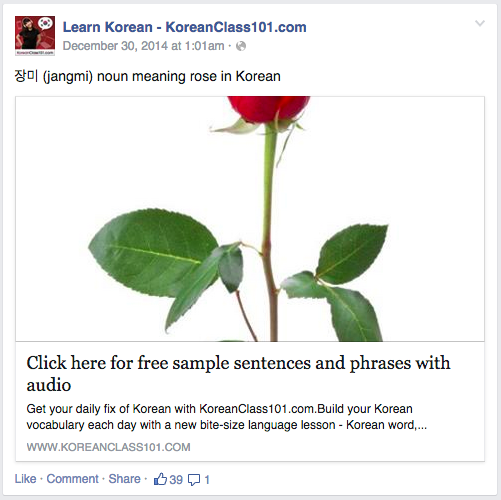
\includegraphics[width=\columnwidth]{learn-korean-post.png}
\caption{An example Daily Word post from KoreanClass101, a Facebook service with 70 thousand subscribers.}
\label{fig:learn-korean}
\end{figure}

% because . These services also generally rely on an external site for 

% ALOE is a system that allows users to learn foreign-language vocabulary while browsing the web, by replacing words in the user's native language with foreign-language vocabulary \cite{augmenting}. This work differs from existing microlearning systems by 

\section{FeedLearn Interface}

FeedLearn is a Chrome extension which inserts small vocabulary quizzes into the user's Facebook feeds.

\subsection{Quiz Types}

These quizzes initially present a noun in the native language, and ask the user to select the corresponding foreign-language word, as shown in \autoref{fig:quiz1}. In order to ensure that users learn to recognize the word associations in both ways, we also have a second type of quiz, in which the user is shown a word in the foreign language and selects the corresponding word in their native language, as shown in \autoref{fig:quiz2}.

\begin{figure}
\centering
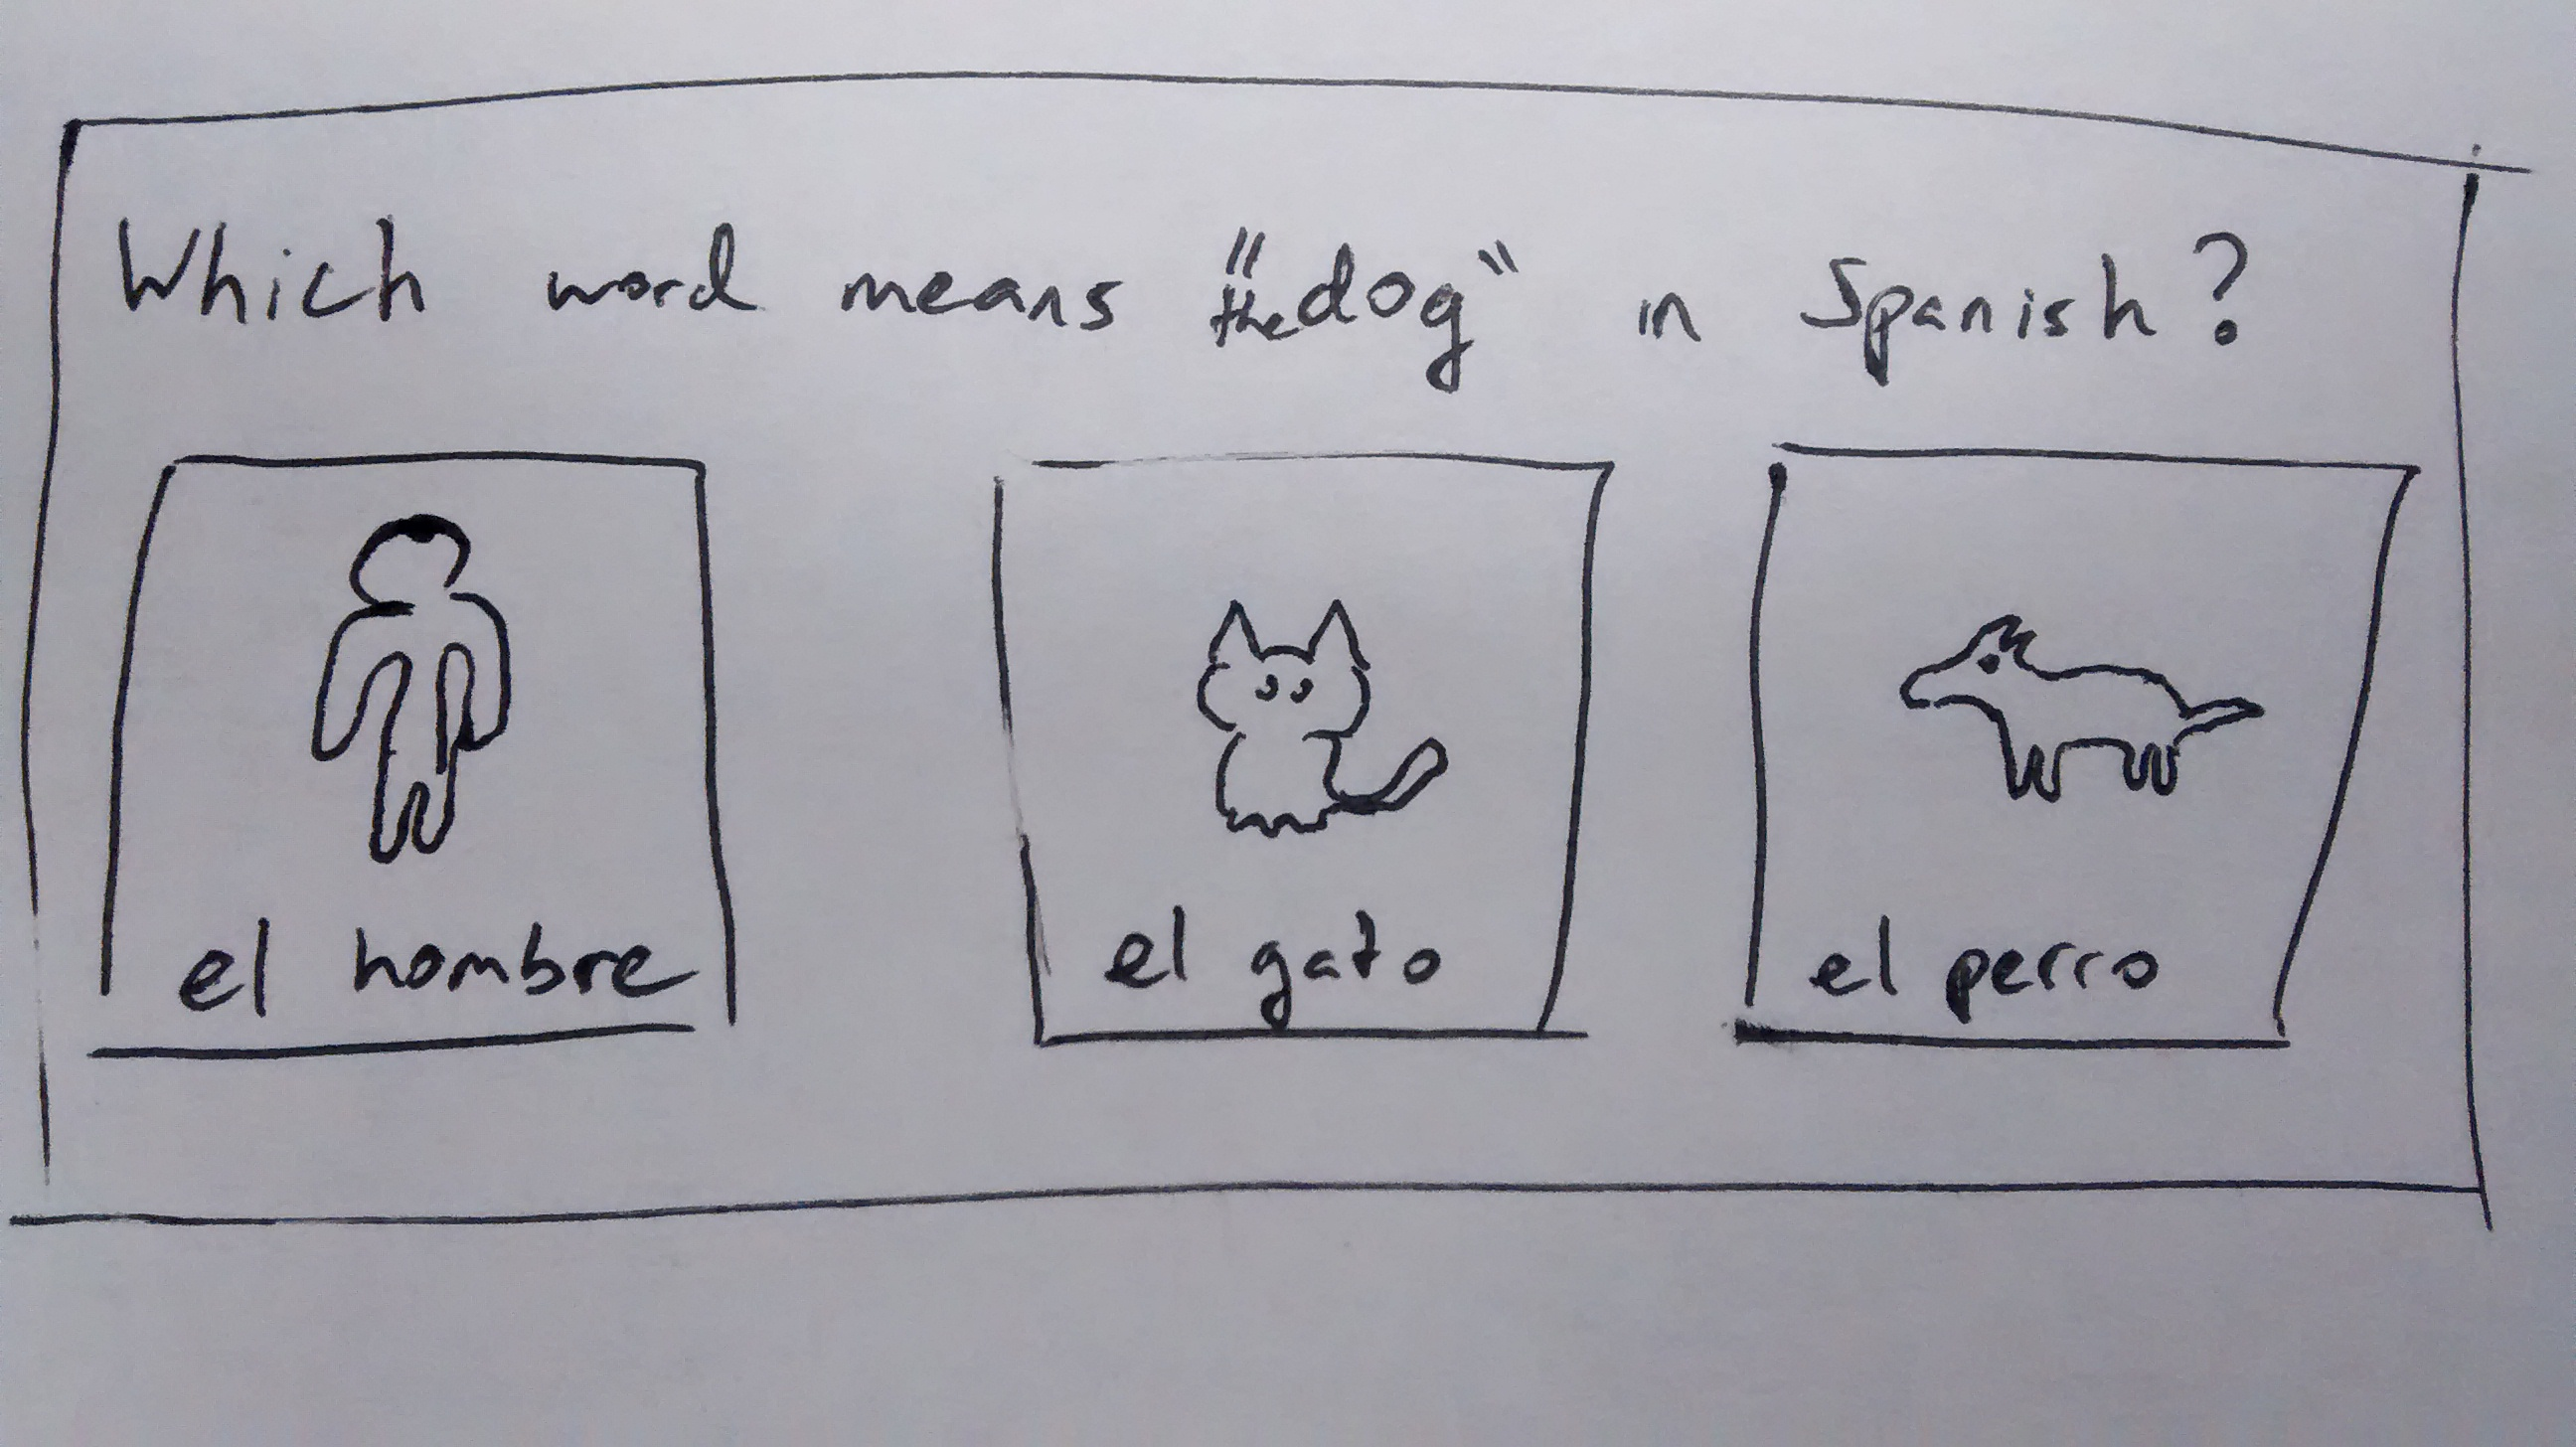
\includegraphics[width=1.0\columnwidth]{quiz1}
\caption{One type of quiz presents a noun in Japanese (\textit{jikan}), and asks the user to select its meaning (time).}
\label{fig:quiz1}
\end{figure}

\begin{figure}
\centering
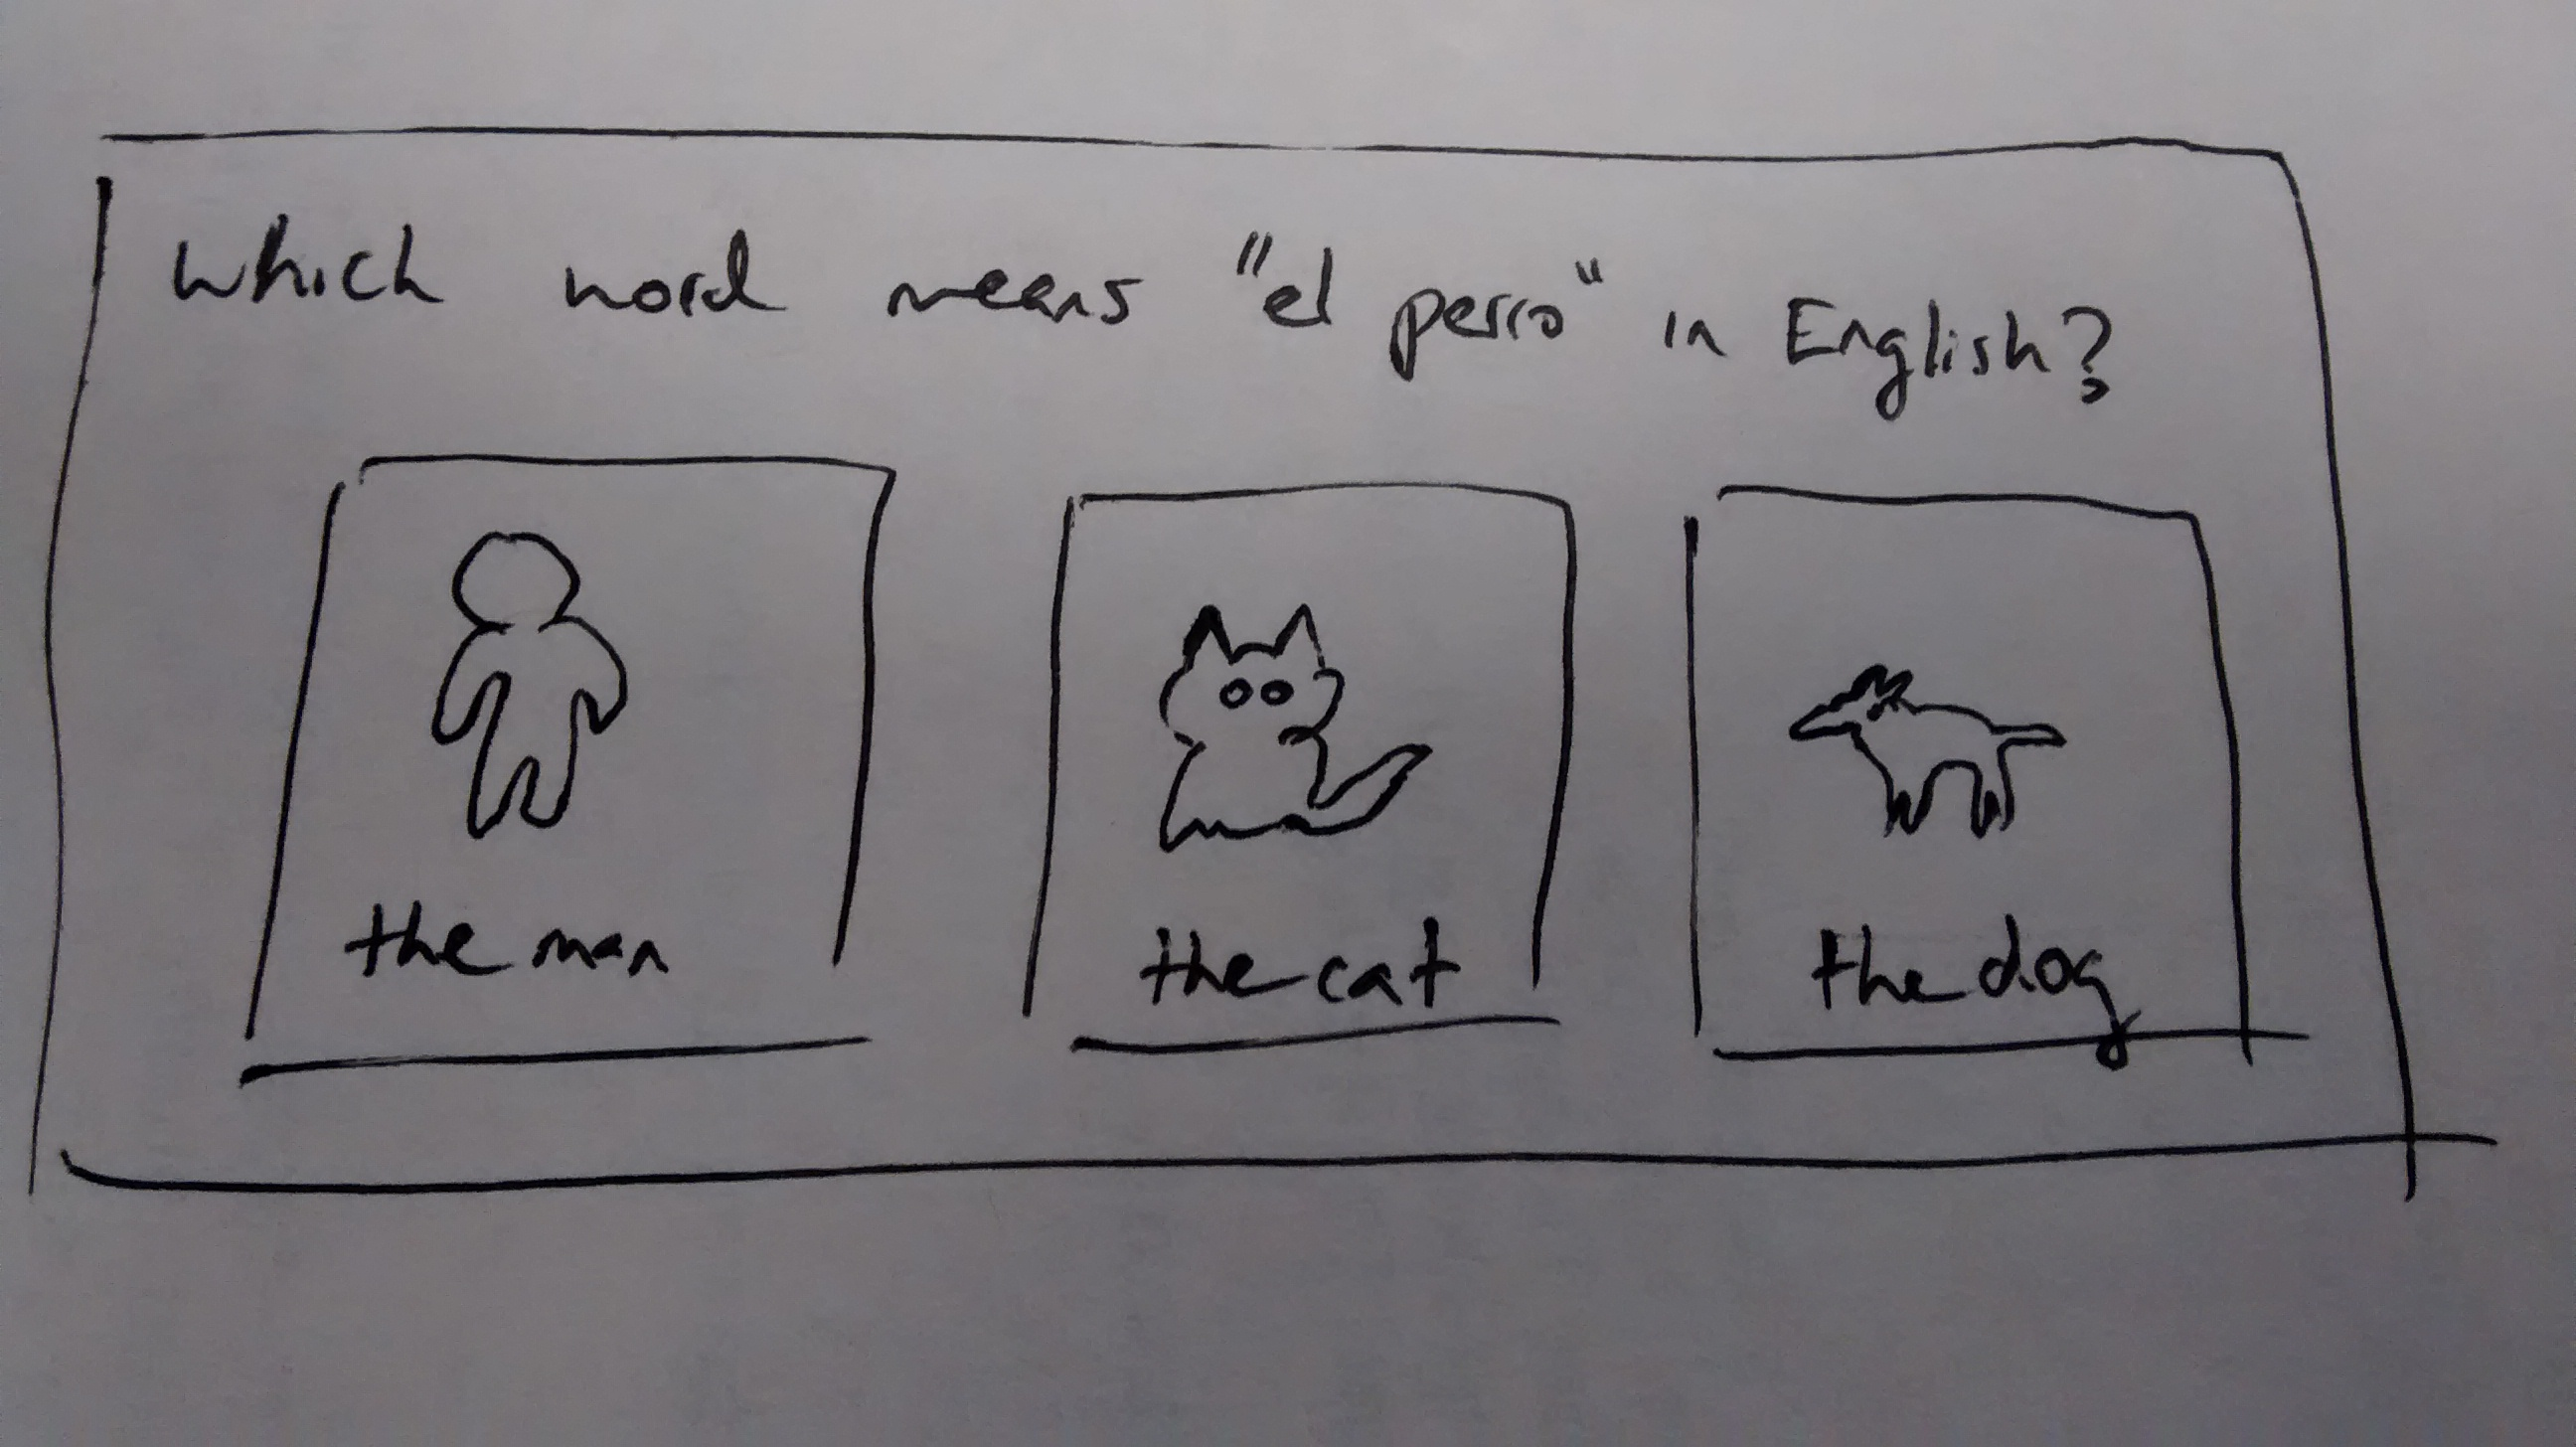
\includegraphics[width=1.0\columnwidth]{quiz2}
\caption{Another type of quiz presents a noun in English (umbrella), and asks the user to select the correct translation into Japanese (\textit{kasa}). The user has incorrectly selected \textit{fukuro}, so the user is shown its meaning (bag), and tries again.}
\label{fig:quiz2}
\end{figure}

Our words and definitions were taken from the Nouns section of Wiktionary's 1000 Basic Japanese Words list. We excluded loanwords that users would easily recognize (\textit{pinku}=pink), and words that are homographs when romanized (\textit{hana}=flower or nose). We focus on nouns, because they are the most common type of word -- the majority of words in the Oxford English dictionary are nouns \cite{microlearning}. FeedLearn can optionally show the word in the native script (kana/kanji for Japanese), or display a picture of the word. However, we did not show these in our user study, because our users could not read Japanese scripts, and not all words can be visualized with a picture (ex: year).

% A picture is also presented alongside the foreign-language word, to help learners visually remember them. Prior research has shown that flashcards showing a picture along with the text allow learners to learn vocabulary better than text-only flashcards \cite{multimediavocabulary}. We focus on nouns, because they are the most common type of word -- the majority of words in the Oxford English dictionary are nouns \cite{microlearning} -- and they are relatively easy to visualize. This is the same quiz style used by Duolingo to introduce nouns.

We opt to use this interactive quiz format, rather than simply showing pairs of words and translations or asking users to explicitly recall and type out translations for words, because it allows us to take advantage of the testing effect with a minimal amount of interaction -- the user simply clicks on a word to answer. If the user clicks the wrong word, . If the user answers a quiz correctly, a new quiz testing a different word is shown. Thus, users can continue to study for as long as they wish to.

\subsection{Quiz Generation}

Quizzes are generated automatically from the provided English word. The other options are generated by looking up the word in WordNet \cite{wordnet}, to find related words that have similar category and semantics but have different meaning (for example, other animal names). The images are obtained by taking the first result on Google Images. We select the list of words to teach based on their overall usefulness in the language (as judged by word frequency in natural-language text).

\subsection{Spaced Repetition}

We use the Memreflex spaced-repetition algorithm to ensure that items are appropriately spaced for review, and new items are introduced only once the user is ready to learn more \cite{memreflex}. However, we show the word due for review that has been seen least recently in the feed, as opposed to always showing the most overdue word as Memreflex does. This ensures that users will continue to see different words as they are scrolling through their feeds, even if they are not always answering the quiz questions.

\subsection{Inserting Quizzes into Feeds}

We insert quizzes into feeds so that they will be encountered at a rate of 1 quiz every 10 posts. We picked this rate, as this was similar to the frequency we observed advertisements and sponsored content appearing in Facebook news feeds. Hence, our should not distract users any more than existing advertisements. %on Facebook. % This is optimal because (need justification).

\section{Evaluation}

We conducted a weeklong between-subjects user study to evaluate the effectiveness of our system in teaching foreign-language vocabulary.

% We conducted a 2-week between-subjects user study to evaluate the effectiveness of our system in teaching foreign-language vocabulary.

\subsection{Participants}

We recruited 13 users who had not previously studied Japanese, who were interested in learning some basic vocabulary. They were voluntary participants recruited from online groups. All of our participants were regular users of Facebook. %, spending at least 10 minutes on the site each day.

% We recruited 30 college students with no prior exposure to Japanese, who were interested in learning some basic vocabulary in Japanese. All of our participants were regular users of Facebook, spending at least 10 minutes on the site each day.

\subsection{Materials}

We selected the 30 most frequently used non-abstract nouns in Japanese, and generated flashcards automatically for them, according to the procedure described in the Quiz Generation section. We presented vocabulary words in romanized form rather than the standard Japanese orthography, to avoid difficulties resulting from unfamiliarity with the Japanese writing system.

\subsection{Conditions}

There were 3 conditions in our study. We assigned 10 students to each:

\begin{itemize}
\item FeedLearn: We inject the quizzes directly into the user's Facebook news feed
\item External Service with In-Feed Reminders: We inject reminders into the news feed asking users to go visit a website where they can take a quiz. The quiz interface on the external website is identical to the one we would have injected directly into the feeds in the FeedLearn condition. The reminders in the feed occur at the same frequency as the quizzes would have been shown in the feeds. This is intended to resemble the experience that would be seen by users using Duolingo and other educational apps, if the users' friends had also enabled posting into their Facebook feeds.
\item External Service with Daily Email Reminders: We give the user a link to the external quizzing service, and send them a daily email at 10AM asking them to go review vocabulary on the site.
\end{itemize}

\subsection{Procedure}

The study is conducted entirely online. First, we ask the users to take a pre-test, to verify that they do not already know the vocabulary that we intend to teach them. The test is a multiple choice test: there are 30 questions total, with 15 questions where questions where the user is given the foreign-language word and is asked to select the correct English translation, and 15 questions where the user is given a word in English and is asked to select the correct foreign translation.

Then, we have them install our extension have them use the service for 2 weeks (according to the condition they have been assigned to). After the 2 weeks have elapsed, we again ask them to take the vocabulary quiz.

\subsection{Research Questions}

H1: Do users learn more vocabulary in the FeedLearn condition than the other conditions?

H2: Do user engage more (complete more quizzes) in the FeedLearn condition than the other conditions?

H3: Do users enjoy the FeedLearn condition more than the other conditions?

\section{Results}

H1: Hopefully, we find that the amount of vocabulary learned in the FeedLearn condition is greater than the other two conditions

H2: Hopefully, we find the users engage more (complete more quizzes) in the FeedLearn condition than the other conditions.

H3: Hopefully, we find that users find injection of quizzes directly into their Facebook feeds less distracting than injection of reminders for them to visit the site, or email-based reminders.

\section{Discussion}

Although in all 3 conditions, users receive daily reminders to go study vocabulary, we found that users complete more quizzes in the FeedLearn condition, and consequently learn more vocabulary.

Relative to the External Service with In-Feed Reminders condition, we can attribute this to the reduced friction required for the interaction: the user no longer needs to leave their news feed and visit an external service to review vocabulary, so the barrier to engagement is lowered by inserting vocabulary quizzes directly into social feeds.

Relative to the External Service with Email Reminders condition, we can additionally attribute an advantage to being able to catch them when they are idle and free. While the user may be busy at 10AM and not have time when they receive the email to review the vocabulary, and will consequently have to remember to go visit the site at a later time, users in the FeedLearn condition have already indicated that they are free and idle because they are browsing their news feed, and are hence more likely to be available to review vocabulary when they encounter them in their feeds.

Users found the FeedLearn condition more enjoyable and less distracting than the External Service with Email Remdiners condition, because they were able to directly go engage with the quiz content, and were not distracted by unnecessary reminder emails.

\section{Conclusion}

Injecting small, actionable tasks into users' Facebook feeds presents an opportunity to influence behavior. Although we have studied foreign-language vocabulary acquisition in this study, our approaches should be equally applicable to other flashcard-like educational content that takes relatively little effort to consume and could be easily injected and interacted with directly inside a social news feed. One could also use a similar mechanism to encourage other behaviors that need to be done for short periods of time on a daily basis, such as small amounts of exercise.

\bibliographystyle{acm-sigchi}
\bibliography{feedlearn}
\end{document}
